\section{Вычислительные эксперименты}

    \subsection{Алгоритм}
        Для реализации моделей сделаем замену переменных \( \beta(t) = \dot{\alpha}(t) \), и получим систему дифференциальных уравнений первого порядка:
        \[
            \begin{cases}
                & \dot{\beta} + w^2 \sin \alpha = 0, \\
                & \beta = \dot{\alpha}, \\
                & \beta(0) = \alpha_1, \quad \alpha(0) = \alpha_0.
            \end{cases} \Rightarrow
            \begin{cases}
                & \dot{\beta} = - w^2 \sin \alpha, \\
                & \dot{\alpha} = \beta, \\
                & \beta(0) = \alpha_1, \quad \alpha(0) = \alpha_0.
            \end{cases}
        \]
        Для системы данного вида можно применять различные численные методы. Уравнения с дополнительными силами аналогично приводятся к такому виду.

        Для компьютерного вычисления будем использовать метод Рунге-Кутты, с помощью которого получим численное решение системы дифференциальных уравнений с заданными параметрами. После чего построим результаты и фазовые плоскости колебаний.



    \subsection{Программа}
        Для расчётов и визуализации был использован язык Python с библиотеками numpy и matplotlib.

        \lstinputlisting[language=Python,
        captionpos=t,
        style=colored,
        basicstyle=\footnotesize\dejavu,
        frame=lines]{src/3model.py}

    \subsection{Результаты}
        Будем строить изменение угла во времени и фазовый портрет системы. Для всех следующих экспериментов длина маятника $L = 1, g = 9.8$, из чего следует, что собственная частота $w = \sqrt{\frac{g}{L}} \approx 3.13\dots$
        \subsubsection{Модель без дополнительных сил}
            Сравним линейное и нелинейное дифференциальное уравнение при различных начальных углах наклона и нулевой начальной скорости.

            \begin{figure}[H]
                \centering
                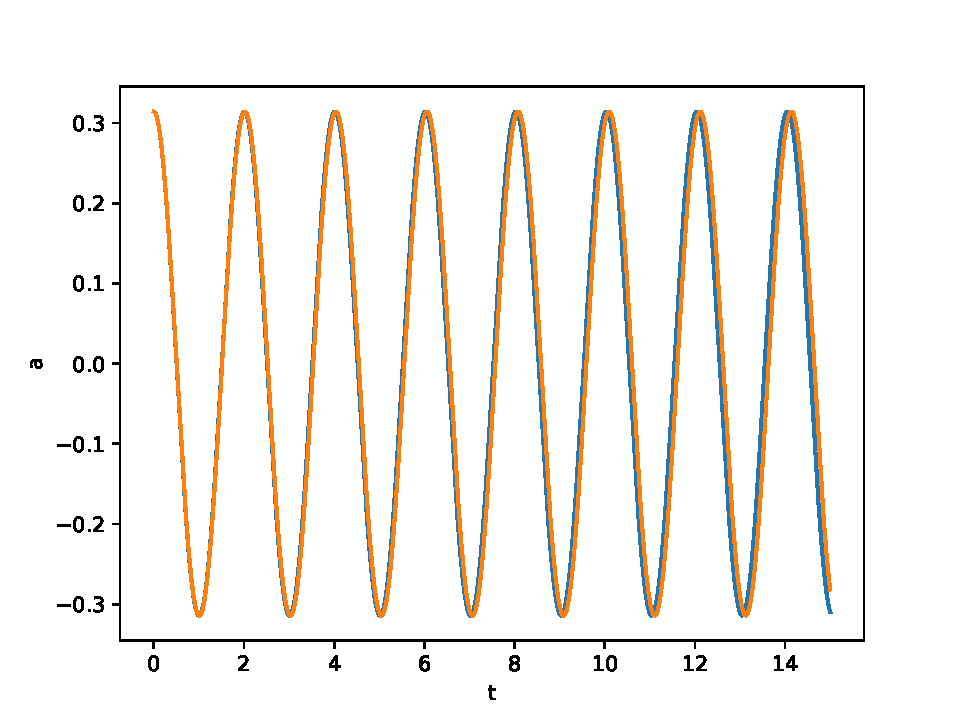
\includegraphics[width=8cm]{pictures/12resonance10.pdf}
                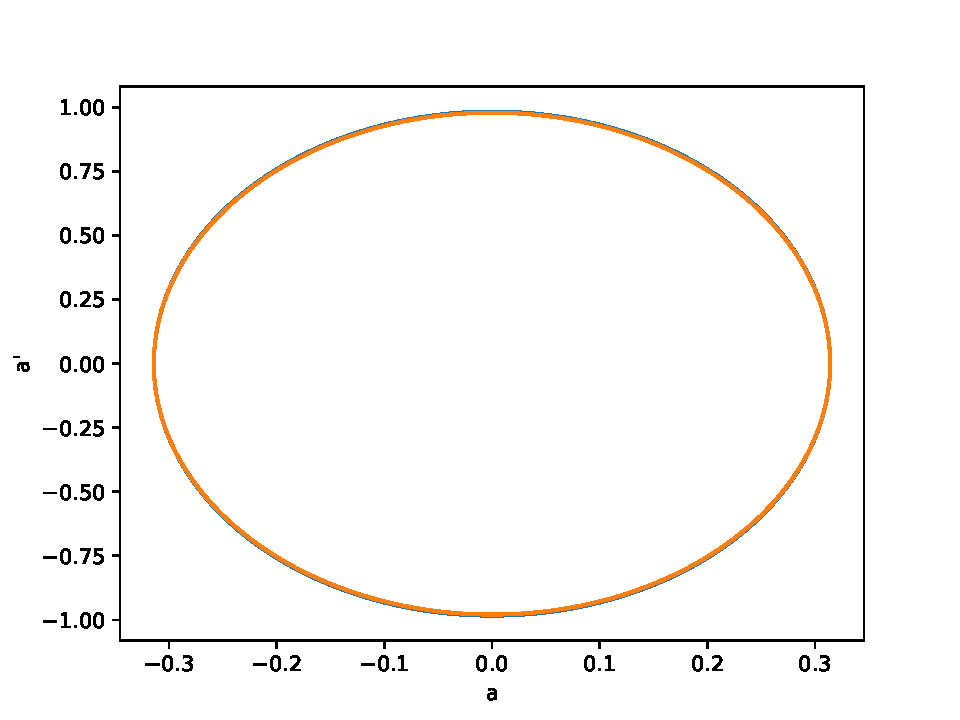
\includegraphics[width=8cm]{pictures/12resonance10p.pdf}
                \caption{$\alpha(0) = \frac{\pi}{10}$.}
            \end{figure}

            \begin{figure}[H]
                \centering
                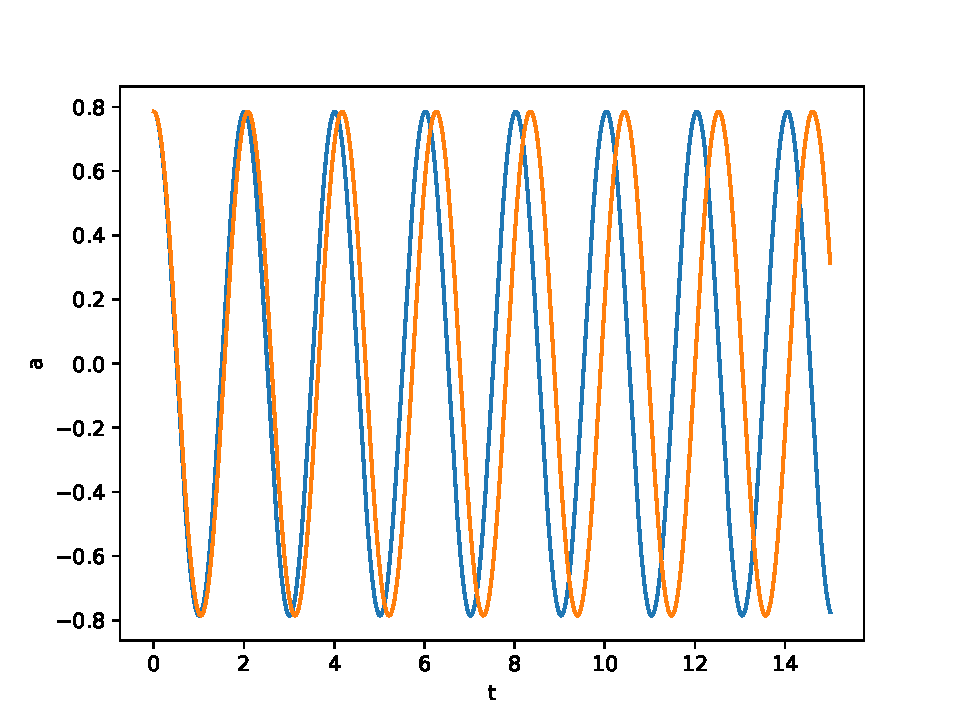
\includegraphics[width=8cm]{pictures/12resonance4.pdf}
                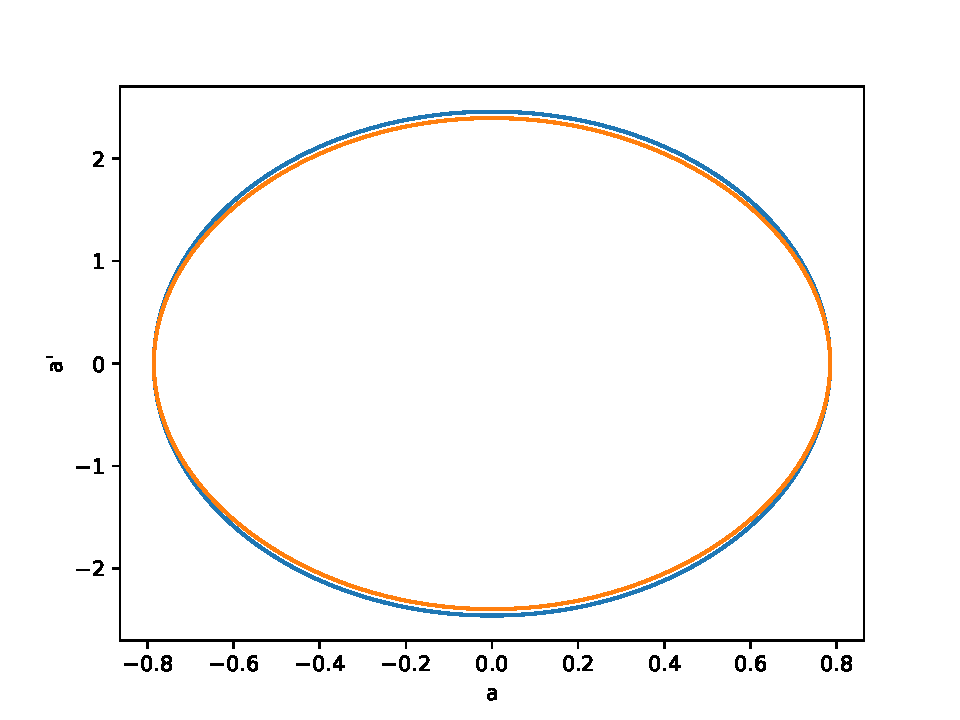
\includegraphics[width=8cm]{pictures/12resonance4p.pdf}
                \caption{$\alpha(0) = \frac{\pi}{4}$.}
            \end{figure}

            Синей кривой визуализирована линейная модель, оранжевой -- нелинейная.
            
            На данных результатах видно, что при небольшом угле наклона разница небольшая, а при большем -- увеличивается период и вместе с этим растёт и погрешность линейной модели. На фазовой плоскости можно увидеть более суженный эллипс у нелинейной модели, что означает меньшую скорость.

        \subsubsection{Модель с трением}
            Рассмотрим результаты влияния трения на маятник.
            \begin{figure}[H]
                \centering
                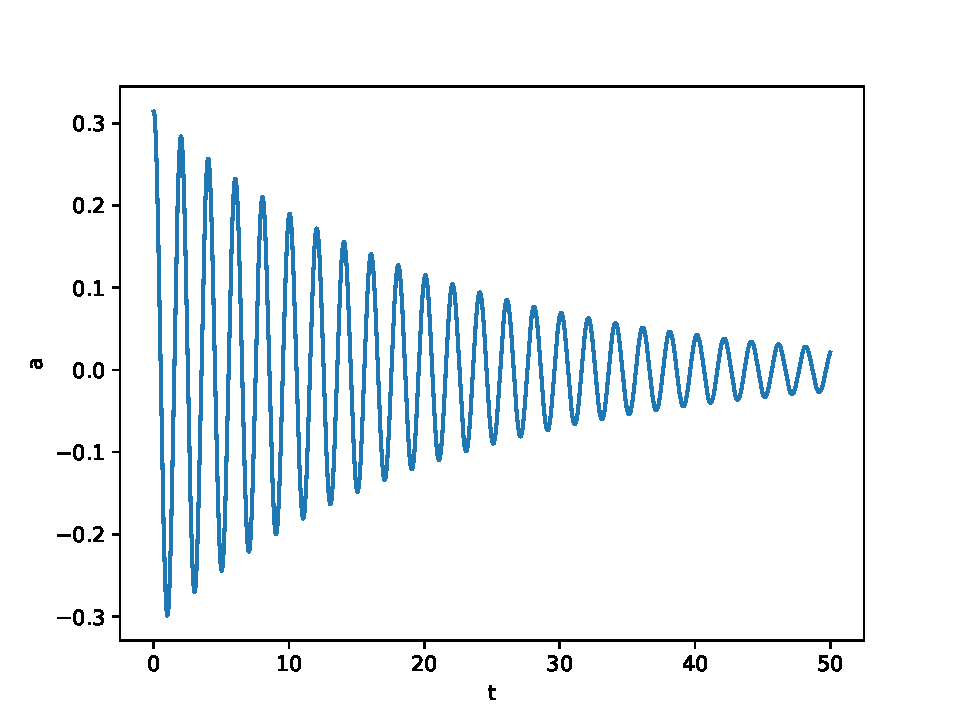
\includegraphics[width=8cm]{pictures/3resonance1.pdf}
                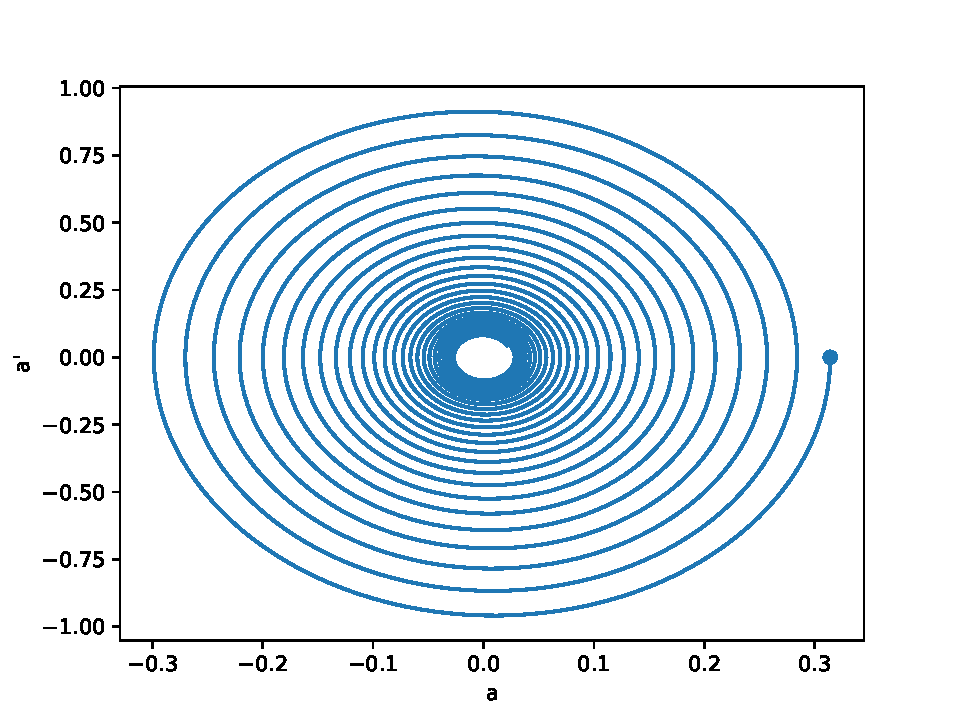
\includegraphics[width=8cm]{pictures/3resonance1p.pdf}
                \caption{$\alpha(0) = \frac{\pi}{10}, ~ \dot{\alpha}(0) = 0, ~ k = 0.1$.}
            \end{figure}
            \begin{figure}[H]
                \centering
                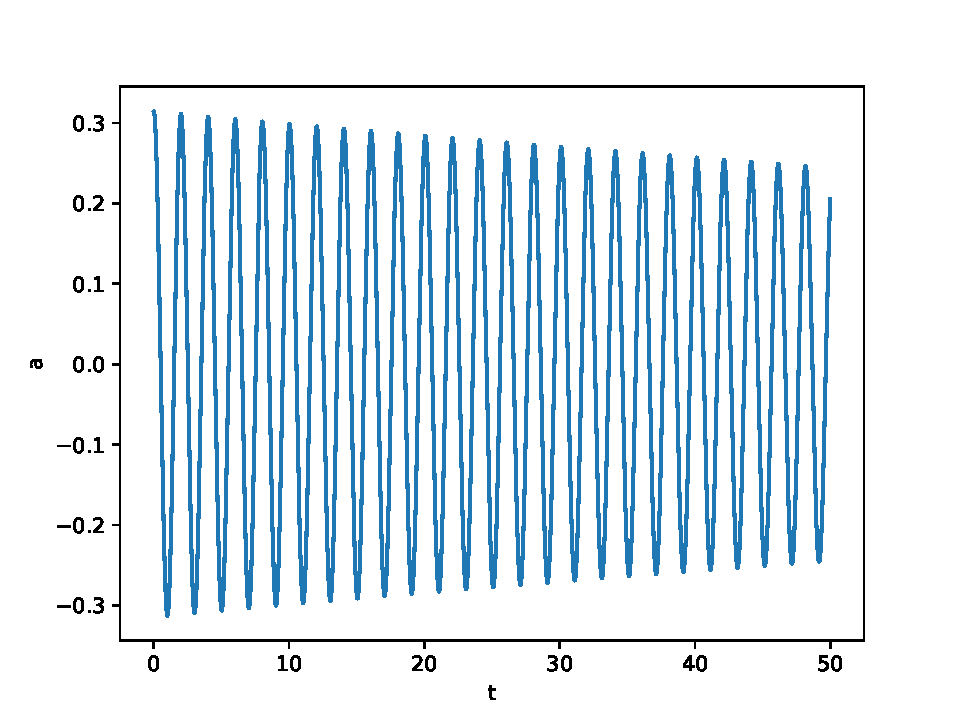
\includegraphics[width=8cm]{pictures/3resonance2.pdf}
                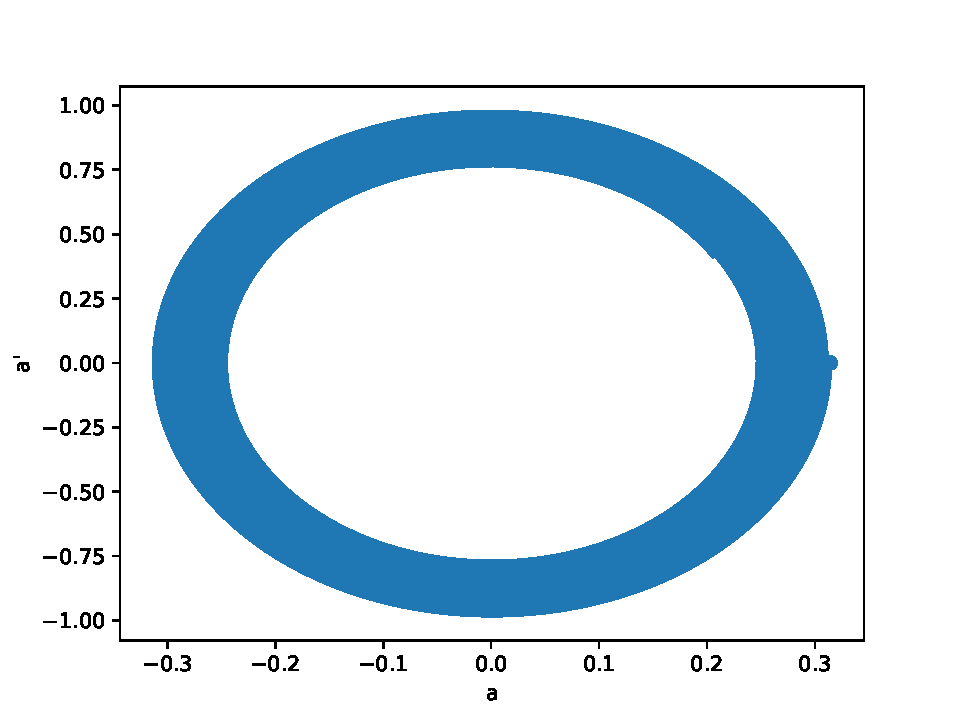
\includegraphics[width=8cm]{pictures/3resonance2p.pdf}
                \caption{$\alpha(0) = \frac{\pi}{10}, ~ \dot{\alpha}(0) = 0, ~ k = 0.01$.}
            \end{figure}

            Видно, что амплитуда колебаний из-за трения со временем уменьшается, поэтому колебания являются затухающими. Кривая на фазовой плоскости из-за затухания постепенно приближается к нулю. Чем меньше коэффициент трения, тем медленнее происходит затухание.

        \subsubsection{Модель с вынуждающими колебаниями}
            Рассмотрим результаты при действии вынуждающих колебаний на маятник с начальными условиями $\alpha(0) = \frac{\pi}{10}, ~ \dot{\alpha}(0) = 0$.
            \begin{figure}[H]
                \centering
                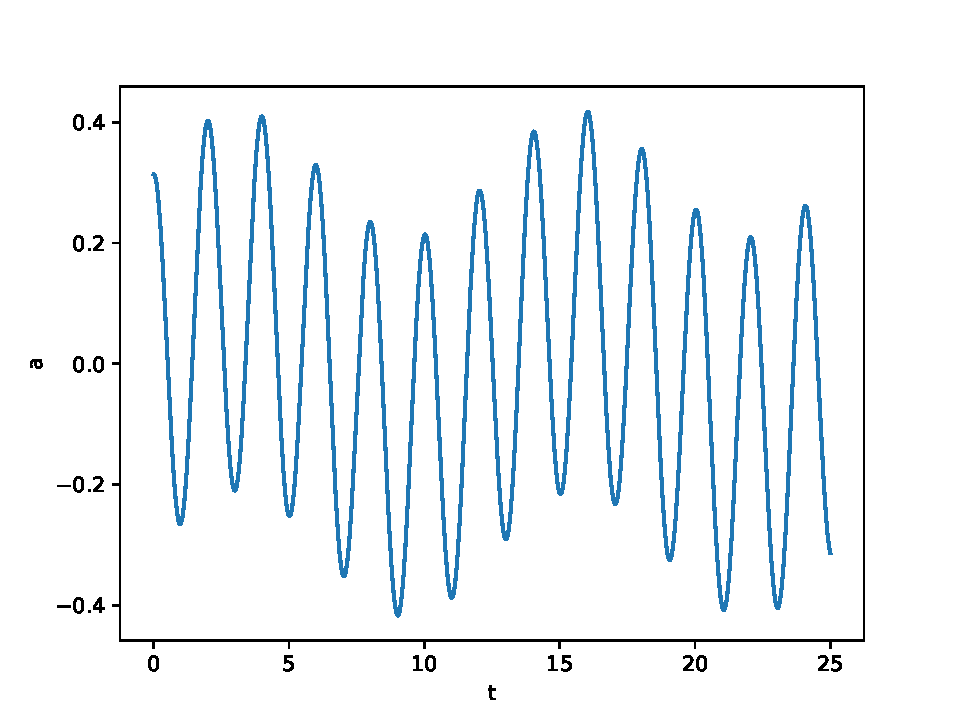
\includegraphics[width=8cm]{pictures/4resonance1.pdf}
                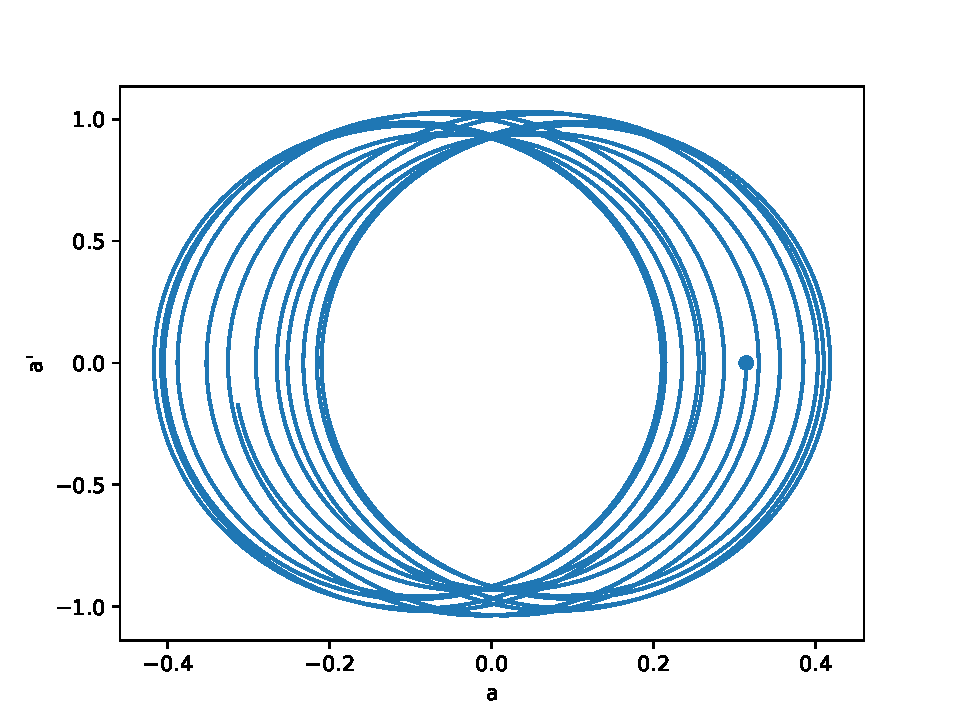
\includegraphics[width=8cm]{pictures/4resonance1p.pdf}
                \caption{$A_f = 1, ~ w_f = 0.5$.}
            \end{figure}
            Из-за вынуждающих колебаний происходит смещение значений угла наклона маятника, что также отражается и на фазовой плоскости.

            \begin{figure}[H]
                \centering
                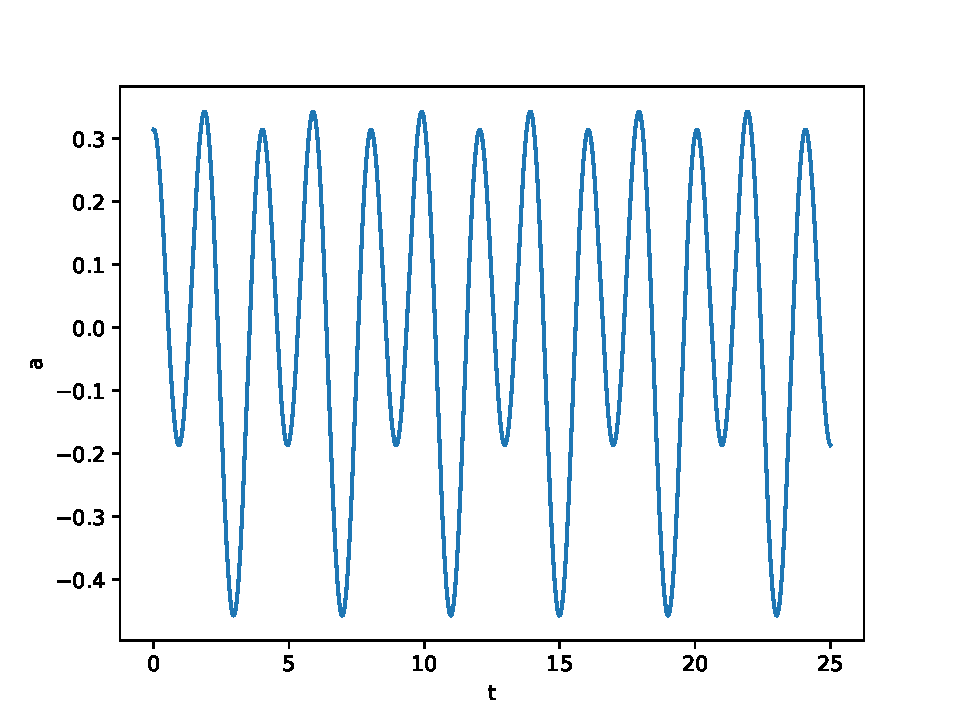
\includegraphics[width=8cm]{pictures/4resonance2.pdf}
                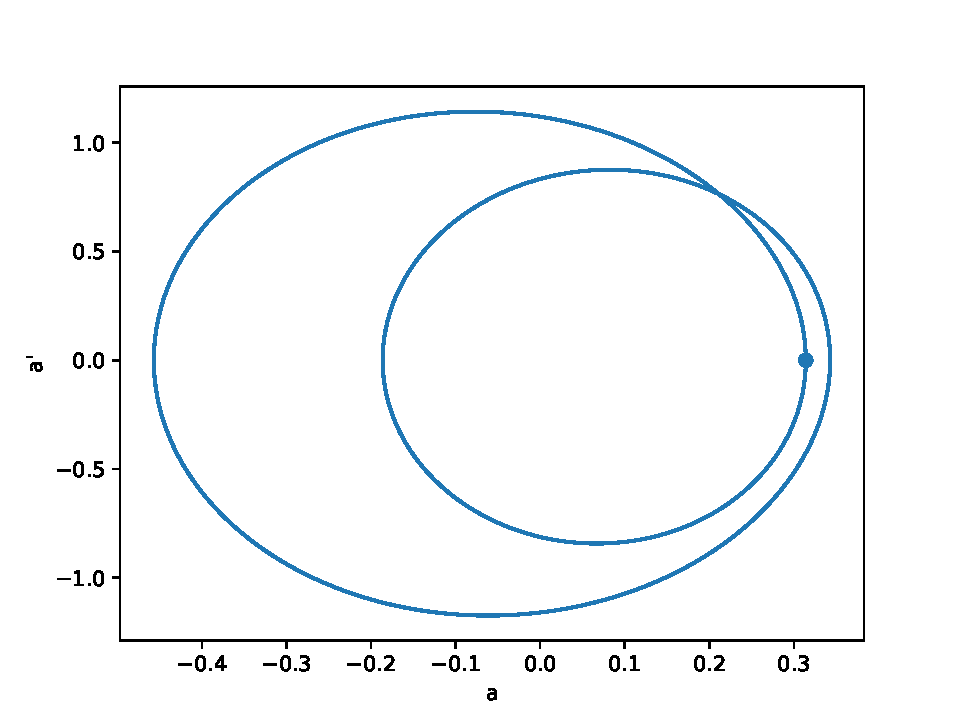
\includegraphics[width=8cm]{pictures/4resonance2p.pdf}
                \caption{$A_f = 1, ~ w_f = \frac{w}{2}$.}
            \end{figure}
            При частоте вынуждающих колебаний, равной целой доли собственной частоты маятника, видно смещение угла, но с некоторым периодом это смещение повторяется. На фазовой плоскости видно замкнутую кривую, что и подтверждает существование некоторого периода колебаний.

            \begin{figure}[H]
                \centering
                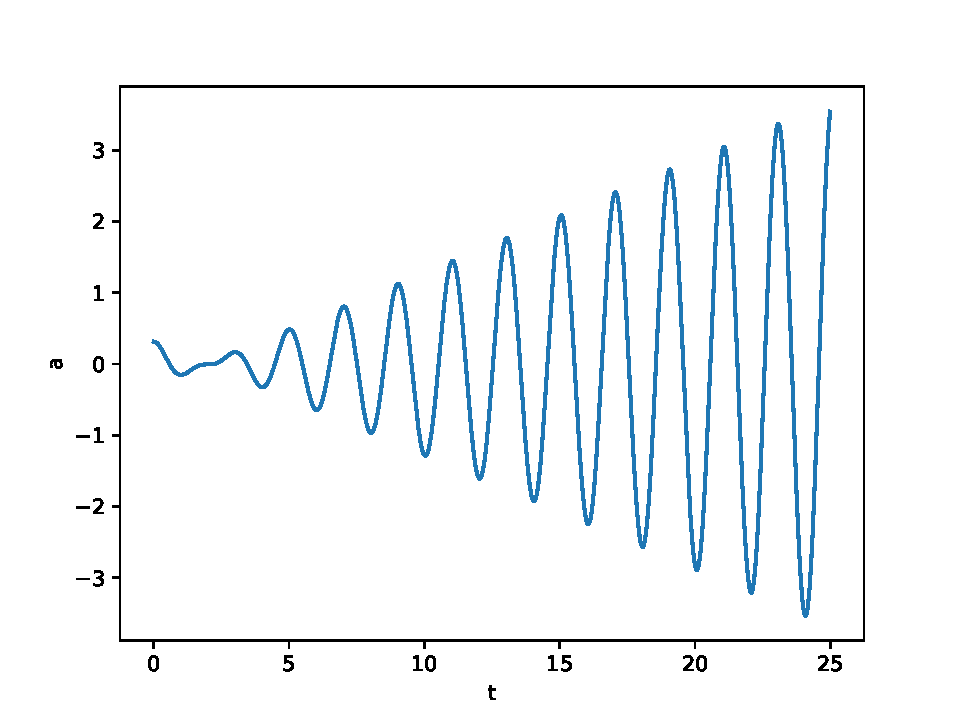
\includegraphics[width=8cm]{pictures/4resonance3.pdf}
                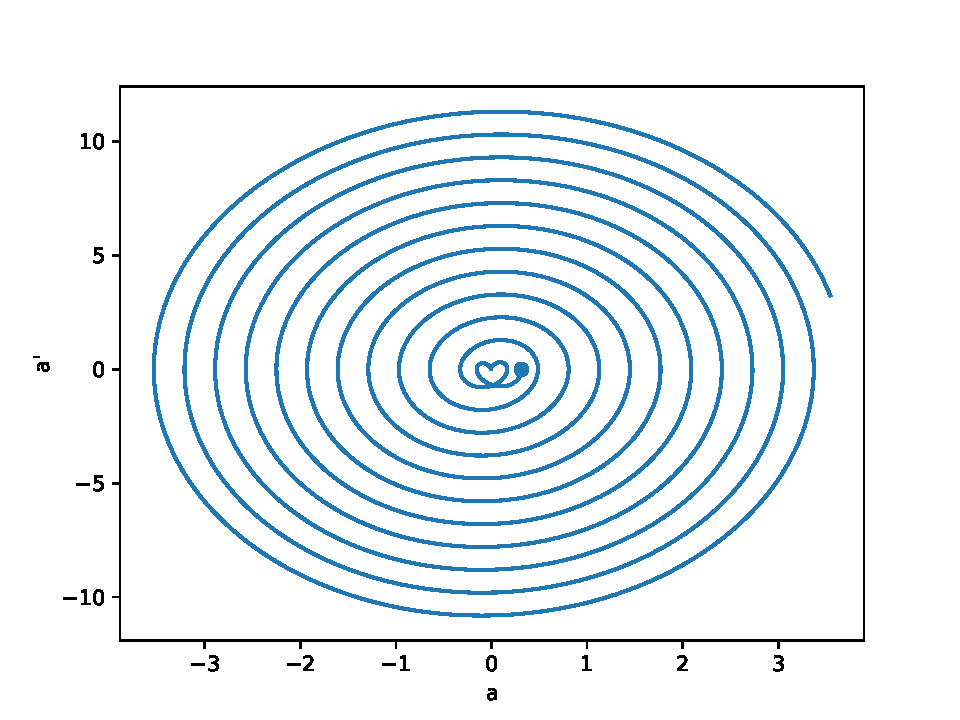
\includegraphics[width=8cm]{pictures/4resonance3p.pdf}
                \caption{$A_f = 1, ~ w_f = w$.}
            \end{figure}
            При совпадении частоты вынуждающих колебаний с собственной частотой маятника происходит эффект резонанса -- амплитуда колебаний неограниченно растёт.

        \subsubsection{Модель с трением и вынуждающими колебаниями}
            Рассмотрим модель, в которой присутствуют обе внешние силы, с начальными условиями: $\alpha(0) = \frac{\pi}{10}, ~ \dot{\alpha}(0) = 0$. Далее синим визуализированы первая четверть данных, а оранжевым -- оставшиеся три четверти.
            \begin{figure}[H]
                \centering
                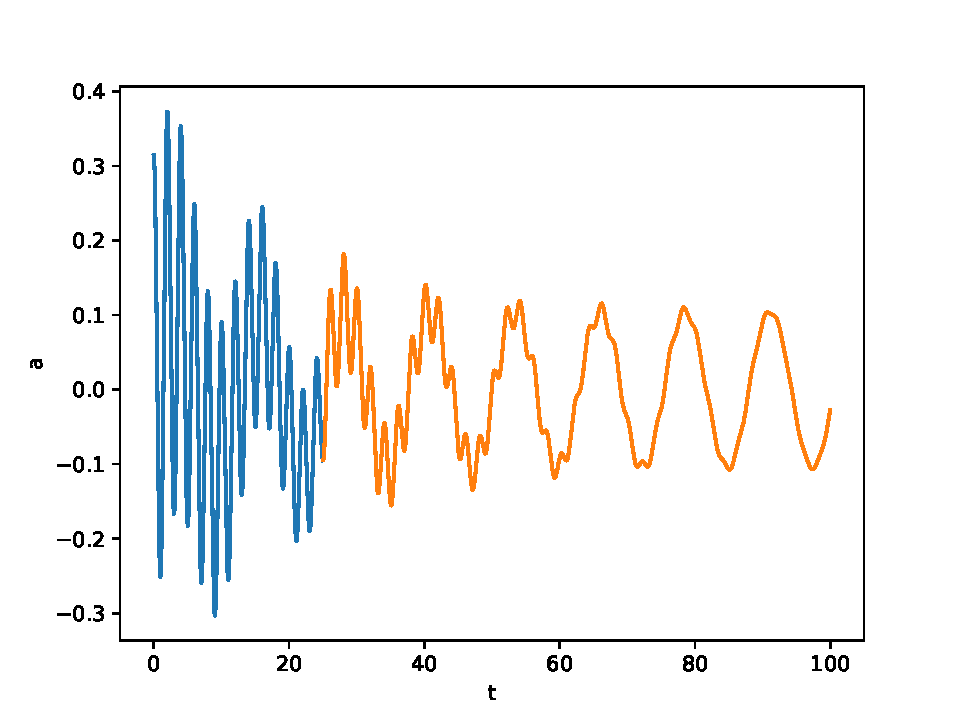
\includegraphics[width=8cm]{pictures/5resonance1.pdf}
                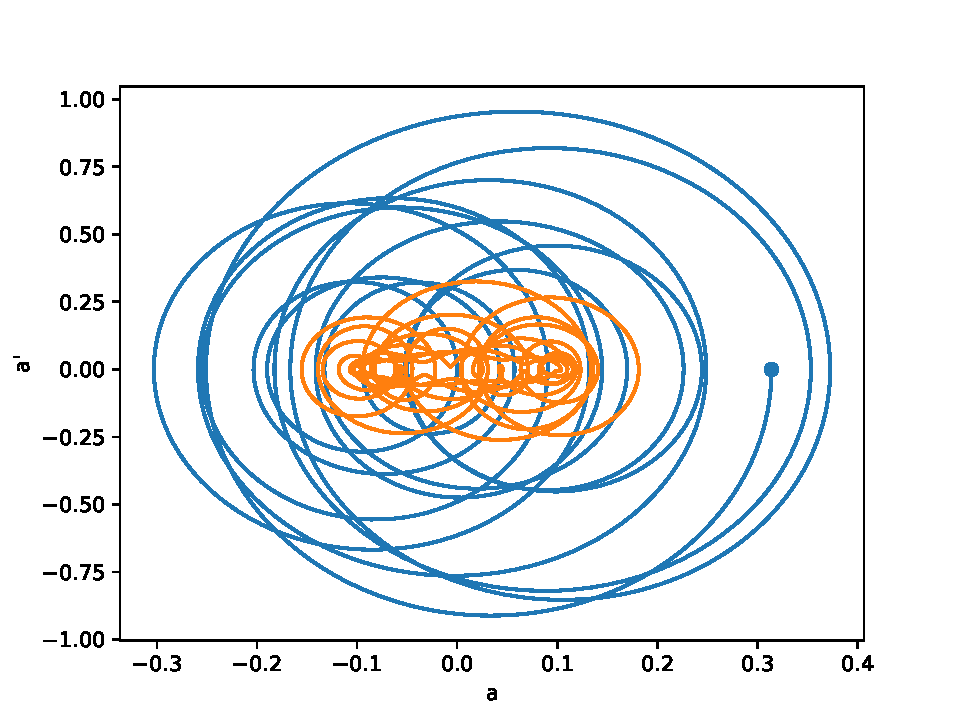
\includegraphics[width=8cm]{pictures/5resonance1p.pdf}
                \caption{$A_f = 1, ~ w_f = 0.5$.}
            \end{figure}
            Изначально хаотическое движение маятника постепенно сглаживается и получается колебание с другим периодом и амплитудой.

            \begin{figure}[H]
                \centering
                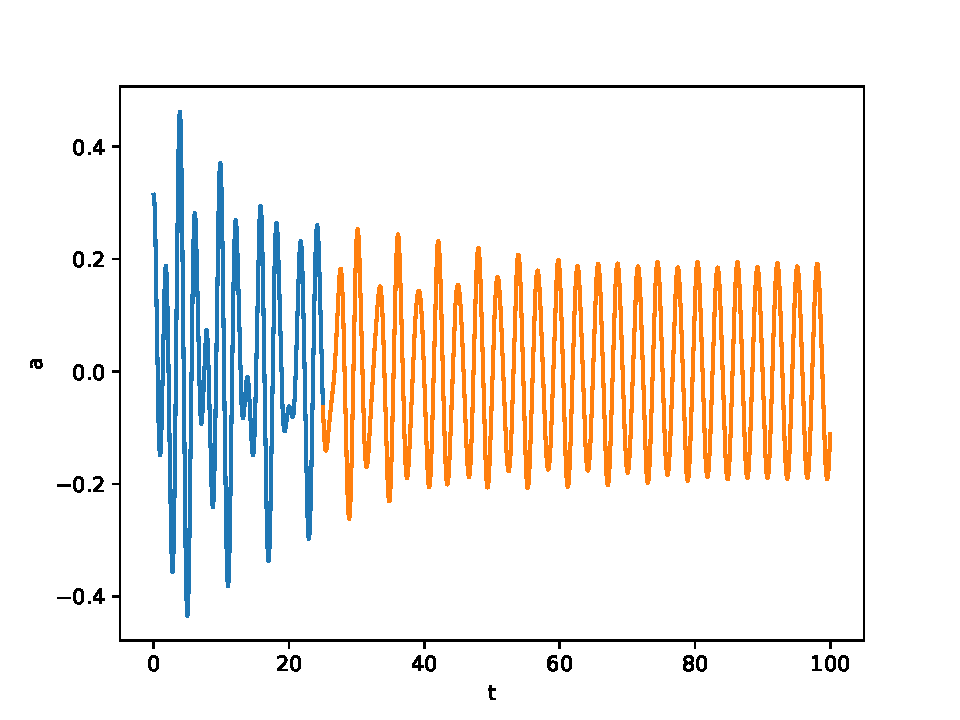
\includegraphics[width=8cm]{pictures/5resonance2.pdf}
                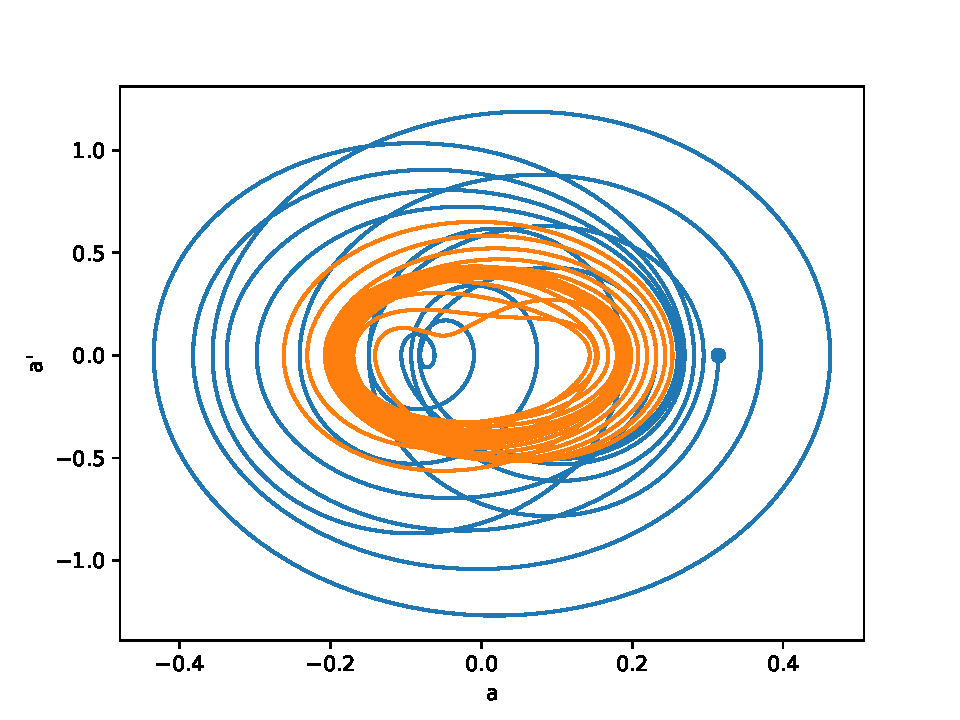
\includegraphics[width=8cm]{pictures/5resonance2p.pdf}
                \caption{$A_f = 1, ~ w_f = w-1$.}
            \end{figure}
            При приближении к собственной частоте период и амплитуда установившихся колебаний увеличиваются.

            \begin{figure}[H]
                \centering
                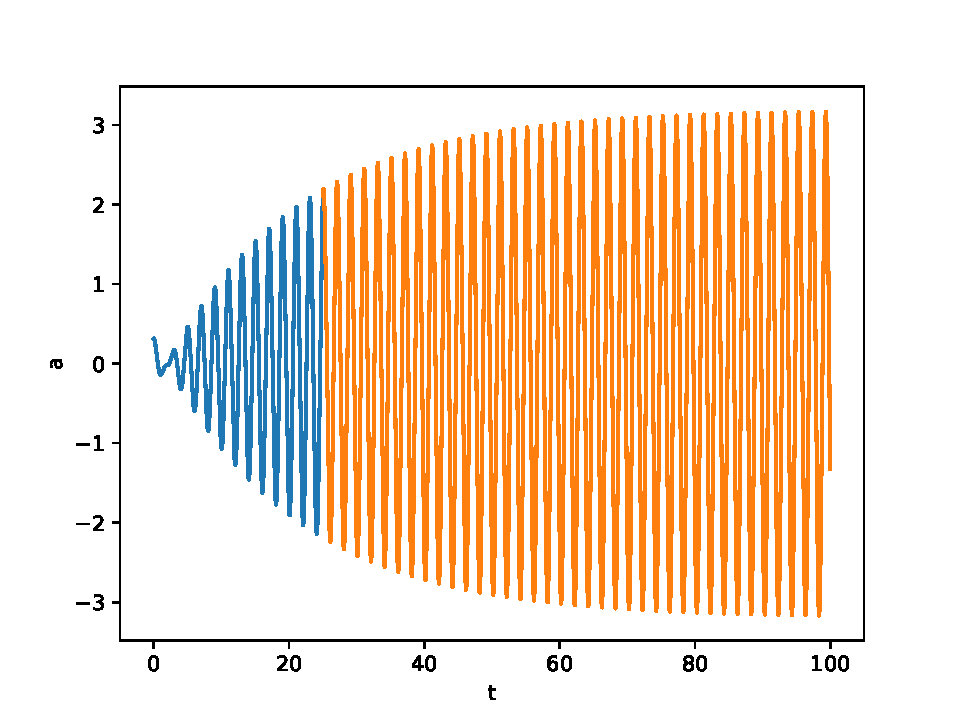
\includegraphics[width=8cm]{pictures/5resonance3.pdf}
                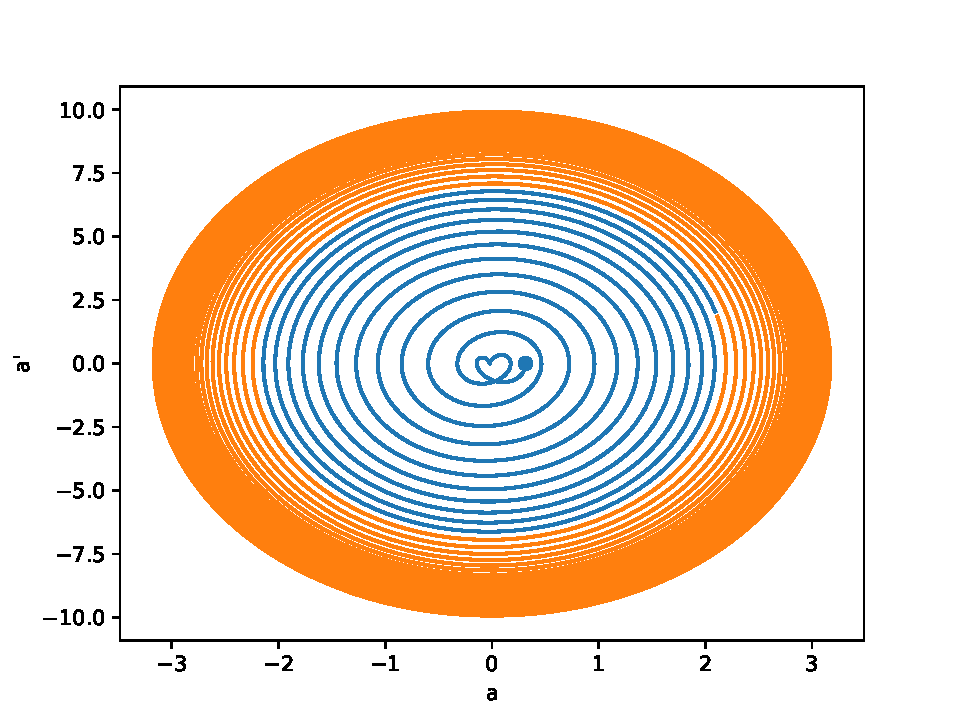
\includegraphics[width=8cm]{pictures/5resonance3p.pdf}
                \caption{$A_f = 1, ~ w_f = w$.}
            \end{figure}
            Самая большая амплитуда достигается при резонансной частоте. В отличие от модели без силы трения, данные резонансные колебания не будут неограниченно увеличиваться. Однако, нельзя делать вывод, что с силой трения резонансная частота является собственной.

        \subsubsection{Резонанс}
            Для того, чтобы исследовать эффект резонанса подробнее построим резонансные кривые. Поскольку этот эффект связан с собственной частотой, будем выбирать несколько значений частоты вынуждающих колебаний около неё. Для каждой такой частоты получим численное решение и найдём из последней четверти значений максимальное по модулю. Получим зависимость \( A = \alpha (w_f) \). Для сравнения с численным решением используем известное аналитическое решение:
            \[
                \alpha (w_f) = \frac{A_f}{~m\sqrt{ \left( 2 w_f w \zeta \right)^2 + \left( w^2 - w_f^2 \right)^2 }~}, \quad \zeta = \frac{k}{2 m w}.
            \]
            В функции используется масса (\( m \)), примем её равной 1.

            По оси \( w \) будем откладывать значения \( \frac{w_f}{w} \) (т.е. резонансная частота находится на отметке 1). Построим кривые для различных значений коэффициента трения на отрезках \( [0.5 w, 2 w] \) и \( [0.9 w, 1.1 w] \). Для выборки значений частоты вынуждающих колебаний возьмём равномерную сетку из 60 точек. 

            \begin{figure}[H]
                \centering
                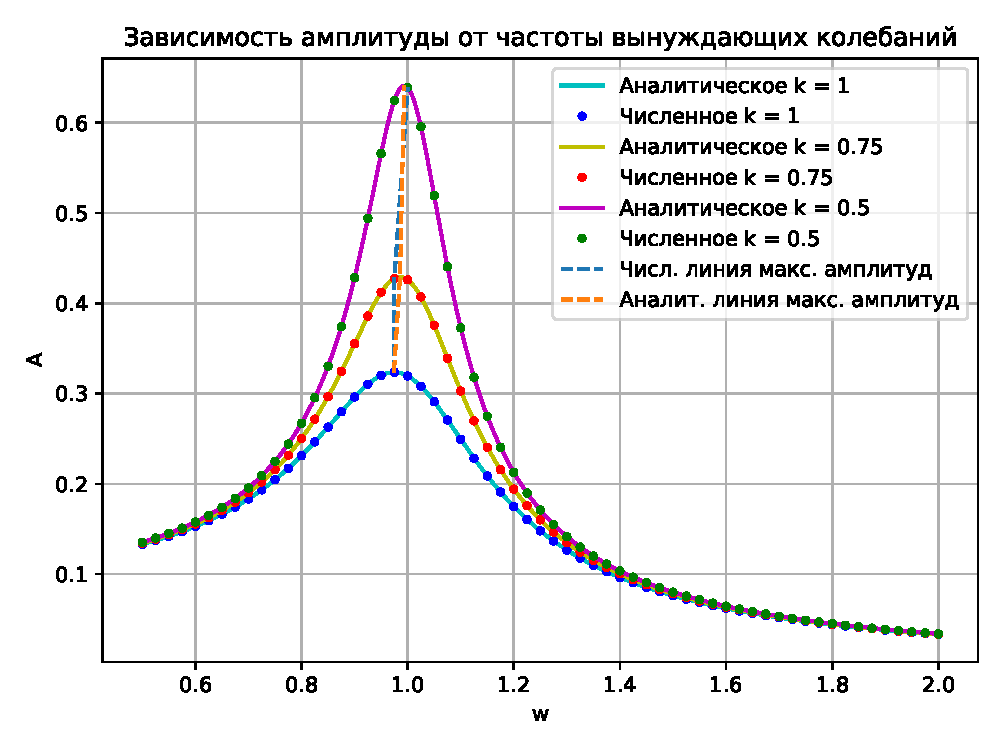
\includegraphics[width=8cm]{pictures/6res05_20.pdf}
                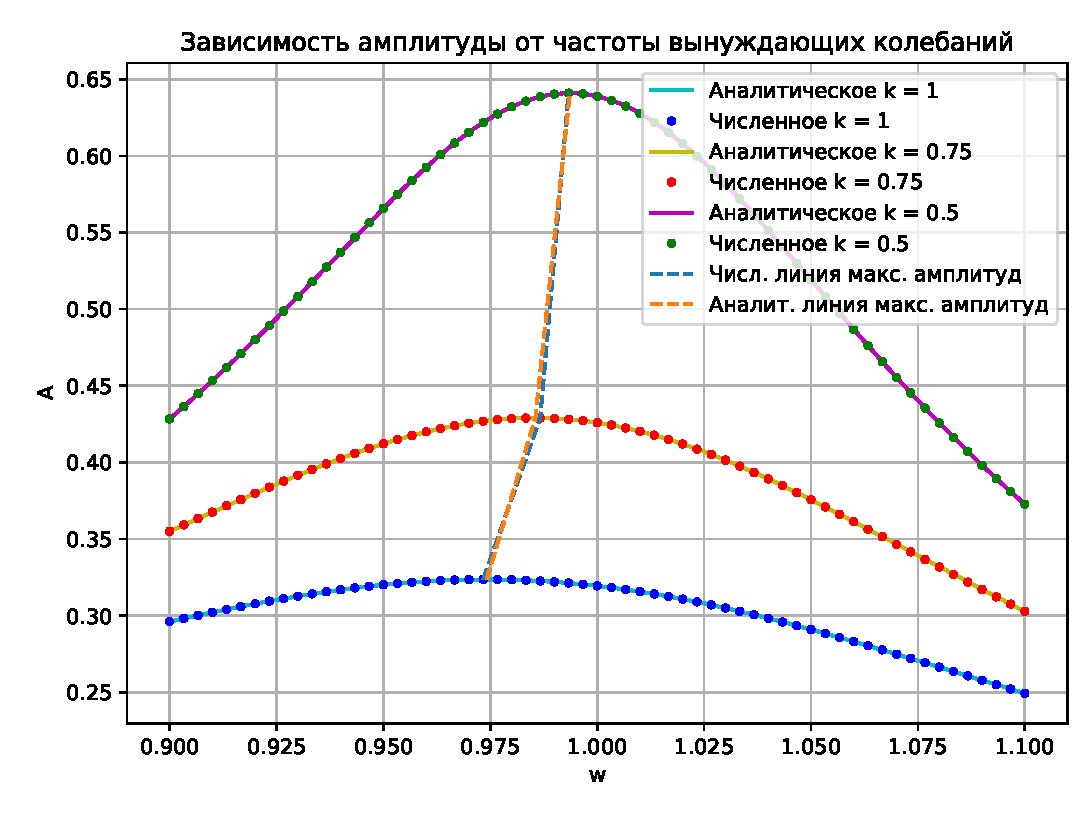
\includegraphics[width=8cm]{pictures/6res09_11.pdf}
                \caption{Кривая амплитуд.}
            \end{figure}
            Видно, что для разных коэффициентов трения резонансная частота достигается в разных местах. При этом, с уменьшением трения амплитуда резонанса становится всё больше, а резонансная частота стремится к собственной.
            